%
% Template for DAS course projects
%
\documentclass[a4paper,11pt,oneside]{book}
\usepackage[latin1]{inputenc}
\usepackage[english]{babel}
\usepackage{amsfonts}
\usepackage{amsmath}
\usepackage{amssymb,amsmath,color}
\usepackage{cite}
\usepackage{graphicx}
\graphicspath{{./figs/}}
\usepackage{float}
\usepackage{tikz}
\usepackage{listofitems} % for \readlist to create arrays
\usepackage[outline]{contour} %
\usepackage{xcolor}

\tikzstyle{node}=[thick,circle,draw=blue,minimum size=22,inner sep=0.5,outer sep=0.6]
\tikzstyle{pixel}=[thick,rectangle,draw=black,fill=white,minimum size=22,inner sep=0.5,outer sep=0.6]
\tikzstyle{node in}=[node,green!20!black,draw=green!30!black,fill=green!25]
\tikzstyle{node hidden}=[node,blue!20!black,draw=blue!30!black,fill=blue!20]
\tikzstyle{node out}=[node,red!20!black,draw=red!30!black,fill=red!20]
\tikzstyle{connect}=[thick,black] 
\tikzset{ % node styles
  node 1/.style={node in},
  node 2/.style={node hidden},
  node 3/.style={node out},
}
\def\nstyle{int(\lay<\Nnodlen?min(2,\lay):3)} % map layer number onto 1, 2, or 3

\usepackage{hyperref}
\hypersetup{
    colorlinks,
    citecolor=black,
    filecolor=black,
    linkcolor=black,
    urlcolor=black
}


\begin{document}
\pagestyle{myheadings}

%%%%%%%%%%% Cover %%%%%%%%%%%
\thispagestyle{empty}                                                 
\begin{center}                                                            
    \vspace{5mm}
    {\LARGE UNIVERSIT\`A DI BOLOGNA} \\                       
      \vspace{5mm}
\end{center}
\begin{center}
  \includegraphics[scale=.27]{logo_unibo}
\end{center}
\begin{center}
      \vspace{5mm}
      {\LARGE School of Engineering} \\
        \vspace{3mm}
      {\Large Master Degree in Automation Engineering} \\
      \vspace{20mm}
      {\LARGE Distributed Autonomous Systems} \\
      \vspace{5mm}{\Large\textbf{DISTRIBUTED CLASSIFICATION VIA NEURAL NETWORKS AND FORMATION CONTROL}}                  
      \vspace{15mm}
\end{center}
\begin{flushleft}                                                                              
     {\large Professors:}\\
     \textbf{\@ Giuseppe Notarstefano} \\
     \textbf{\@ Ivano Notarnicola} \\        
     \vspace{13mm}
\end{flushleft}
\begin{flushright}
      {\large Students:}\\
      {Simone Cenerini} \\
      {Giulia Cutini} \\
      {Riccardo Paolini} \\
\end{flushright}        %capoverso allineato a destra
\begin{center}
\vfill
      {\large Academic year \@2022/2023} \\
\end{center}



\newpage
\thispagestyle{empty}

%%%%%%%%%%% Abstract %%%%%%%%%%%%
\begin{center}
\chapter*{}
\thispagestyle{empty}
{\Huge \textbf{Abstract}}\\
\vspace{15mm}
\end{center}

\tableofcontents \thispagestyle{empty}
% \listoffigures\thispagestyle{empty}

%%%%%%%%%% Introduction %%%%%%%%%%
\chapter*{Introduction}
\addcontentsline{toc}{chapter}{Introduction}
\section*{Motivations} 

\section*{Contributions}



%%%%%%%%%% Chapter Title %%%%%%%%%%
\chapter{Distributed classification via Neural Network}

\begin{figure}
	\centering
	\includegraphics[scale=0.5]{mnist}
	\caption{Example of images from the \texttt{mnist} dataset}
	\label{mnist}
\end{figure}


In the first task we were asked to correctly classify a set of grayscale images. The dataset, downloaded from the Keras \texttt{mnist}, collects images of hand-written digits of $28\times28$ pixels each one, an example in figure \ref{mnist}. In order to perform our task we were asked to implement a distributed classification: given a predefined number of agents running each one a neural network with the same structure, we were asked to implement a Gradient Tracking algorithm to ensure consensus of the connection weights of the several neural networks runned separately by different agents.

\section{Initial setup}
The first step was to prepare the dataset by a reshape and a normalization of the images. We have flattened the $28\times28$ pixels grayscale images in order to obtain a $[784,1]$ column vector and we have normalized the pixels' intensities by dividing each intensity by $255$ in order to avoid a saturation of the activation function.

The classification we were asked to perform was a binary one: we have choose one among the ten digits (named as \texttt{target}) and assigned to it the label $1$, while, to all the other images, we have assigned the label $0$, in the following way:
\begin{equation}
y_i = 
\begin{cases}
1, & \text{if label = \texttt{target}} \\
0, & \text{otherwise}
\end{cases}
\end{equation}

As a consequence, we have performed a \textbf{balancing of the dataset}: in order to efficiently train our neural network we have equalized the representation of both the classes in the dataset ($50 \%$ of both since we have two classes). In order to do that we have undersampled the number of samples in the majority class. 

\section{Neural Network structure}

% NEURAL NETWORK SCHEME
\begin{figure}
\centering
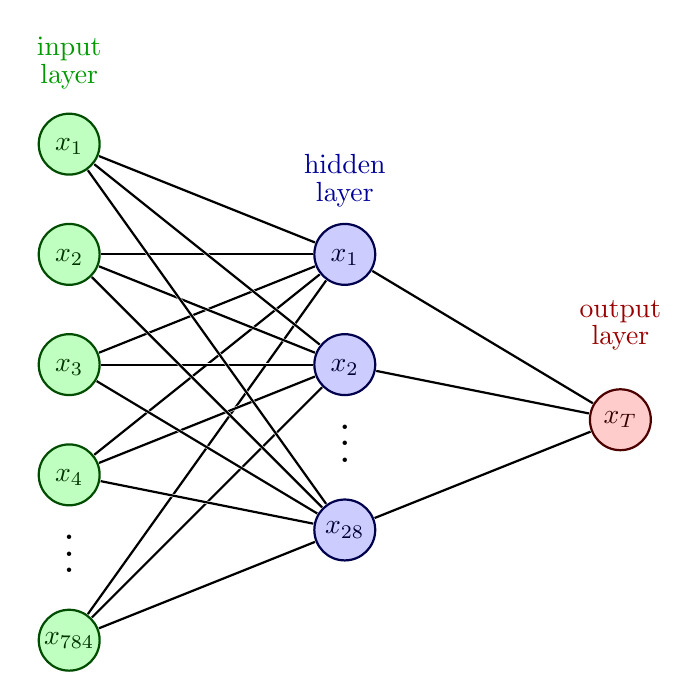
\begin{tikzpicture}[x=3.5cm,y=1.4cm]

\readlist\Nnod{5,3,1} % array of number of nodes per layer
\readlist\Nstr{n,m,k} 
\readlist\Cstr{\strut x,\strut x,{}} 
\def\yshift{0.5} % shift last node for dots


\foreachitem \N \in \Nnod{ 
\def\lay{\Ncnt} 
\pgfmathsetmacro\prev{int(\Ncnt-1)}
\message{\lay,}
\foreach \i [evaluate={\c=int(\i==\N); \y=\N/2-\i-\c*\yshift;
\index=(\i<\N?int(\i):"\Nstr[\lay]");
\x=\lay; \n=\nstyle;}] in {1,...,\N}{


% NODES
\ifnum\lay=1 % First Layer
  \ifnum\i=\N % Last neuron of first layer
    \node[node \n] (N\lay-\i) at (\x,\y) {$x_{784}$}; 
  \else
    \node[node \n] (N\lay-\i) at (\x,\y) {$\Cstr[\lay]_{\index}$};
  \fi
\fi

\ifnum\lay=2 % Second Layer
  \ifnum\i=\N % Last neuron of second layer
    \node[node \n] (N\lay-\i) at (\x,\y) {$x_{28}$}; 
  \else
    \node[node \n] (N\lay-\i) at (\x,\y) {$\Cstr[\lay]_{\index}$}; %empty
  \fi
\fi

\ifnum\lay=3 % Third Layer
  \node[node \n] (N\lay-\i) at (\x,\y) {$x_T$}; 
\fi
      % CONNECTIONS
      \ifnum\lay>1 % connect to previous layer
        \foreach \j in {1,...,\Nnod[\prev]}{ 
          \draw[connect,white,line width=1.2] (N\prev-\j) -- (N\lay-\i);
          \draw[connect] (N\prev-\j) -- (N\lay-\i);
        }
      \fi % nothing to connect first layer
      
    }
\ifnum\lay<\Nnodlen % draw dots for all layers except the last one
    \path (N\lay-\N) --++ (0,1+\yshift) node[midway,scale=1.5] {$\vdots$};
    \fi
}

%%PIXELS
%% Place pixels upstream of the first layer
%\foreach \i in {1,...,\Nnod[1]}{
%  \node[pixel] (P\i) at (0,\Nnod[1]/2-\i) {$p_\i$};
%  \draw[connect] (P\i) -- (N1-\i);
%}
%  
  % LABELS
% \pixel[above=5,align=center,black] at (N1-1.90) {flatten\\[-0.2em]image}
  \node[above=5,align=center,green!60!black] at (N1-1.90) {input\\[-0.2em]layer};
  \node[above=2,align=center,blue!60!black] at (N2-1.90) {hidden \\[-0.2em]layer};
  \node[above=10,align=center,red!60!black] at (N\Nnodlen-1.90) {output\\[-0.2em]layer};
  
\end{tikzpicture}
\caption{Scheme of the neural network for image classification}
\label{NN_scheme}
\end{figure}


The structure we have choose to develop for the neural network is a tapered one, represented in figure \ref{NN_scheme}. 
The first layer is composed by $784$ neurons, that is the dimension of the flattened image we give as input in the network. In this way each neurons of the first layer gets a single pixel as input. The second layer, the hidden one, has $28$ neurons since an higher number of neurons was useless in order to accomplish our task, while it increases a lot the computational effort required to train the network. The last layer has just one single neuron since we are asked to perform a binary classification, and so just a number between $0$ and $1$ is required as prediction.







\chapter{Formation Control} 
 In the second task we were asked to implement in ROS2 a discrete-time version of a \textbf{formation control law} for a team of $N$ robots.

\section{Distance-based formation}
The aim of the task was to obtain a desired geometric formation among a group of $N$ autonomous agents, by acting on the relative positions of agents.

\bigskip
The desired formation can be encoded in terms of an undirected graph, called \textit{formation graph}, whose set of vertices is indexed by the team agents $\mathcal{N} =\{ 1, \cdots, N\}$, and whose set of edges $E=\{(i,j) \in \mathcal{N} \times \mathcal{N} | \, j \in \mathcal{N}_i\}$ contains pairs of agents. Each edge $(i,j) \in E$ is assigned a scalar parameter $d_{ij} = d_{ji} > 0$, representing the distance at which agents $i,j$ should converge to. 

An example could be a predefined formation with hexagon shape with the following \textit{distances matrix}:
\begin{equation}
d_{ij} =
\begin{bmatrix}
0 & l & 0 & d & h & l \\
l & 0 & l & 0 & d & 0 \\
0 & l & 0 & l & 0 & d \\
d & 0 & l & 0 & l & 0 \\
h & d & 0 & l & 0 & l \\
l & 0 & d & 0 & l & 0
\end{bmatrix}
\end{equation}
The desired distance value serve as reference value for the control law. The control law computes control signals for each agent based on its current position and the position of the neighboring agents, aiming to drive the agents towards the desired formation.
The neighbors of a certain agent $i$ can be extracted from the $i$-th row of the distances matrix, by taking the indexes of the elements with $d_j > 0$.

By denoting the position of agent $i \in \{1, \cdots, N\}$ at time $t>0$ with $x_i(t) \in \mathbb{R}^3$, one way to approach distance-based formation control involves the usage of \textbf{potential functions}, similar to the following one:
\begin{equation}
V_{ij}(x)  = \frac{1}{4} \bigg( \lVert x_i - x_j \rVert^2 - d_{ij}^2 \bigg)^2
\label{Formation_potential}
\end{equation}

This kind of potential function represents the energy associated with the relative positions of the agents. By minimizing this potential function, the agents can achieve and maintain the desired formation.
As a consequence, the control law we have implemented for each agent $i$ is the following:
\begin{equation}
\dot{x}_i(t) = f_i(x(t)) = - \sum_{j \in \mathcal{N}_i} \bigg( \lVert x_i - x_j \rVert^2 - d_{ij}^2 \bigg) (x_i - x_j )
\end{equation}

Since we were required to work in discrete time, we denote with $p_i^k \in \mathbb{R}^3$ the discretized version of $x_i(t)$ at time $k$ and, once we have computed the dynamics update for agent $i$ we discretize with Euler formula in the following way:
\begin{equation}
p_i^{k+1} = p_i^{k} + \Delta f_i(p^k)
\end{equation}
where $\Delta > 0$ is the sampling period.

\section{ROS2 implementation}
The solution proposed in previous section has been implemented in ROS2 environment with a code written in Python language.

\bigskip
By means of a launch file (named \texttt{formation\_control.launch.py}) we can generate the desired number of agents and give them the required informations in order to accomplish the target formation. In particular for each agent the launch file generates a ROS2 node that executes the file named \texttt{the\_agent.py}. Each node gets the following main parameters from the launch file:
\begin{itemize}
\item id: a number from $0$ to $N$ associated to the agent's identity
\item initial position, randomly generated
\item distances: each agent gets only "its" row of the distances matrix. In this way it will be able to know who are its neighbors and the distances he has to keep from them in the desired configuration
\item maximum number of dynamics update
\end{itemize}
This file manages the dynamic evolution of the agent and the communication with the other ones (the neighbors' ones). For what regards the communication, we have used a publisher-subscriber protocol implemented in ROS2: each node communicates its position only to its neighbors. The communication between nodes is made using a topic for each edge defined in the formation graph. In order to write to a topic or to read from it, the node must know the name of the topic he want to access.

\bigskip
We have developed also a plotter agent (\texttt{the\_plotter.py}) that can read from its topic the actual positions of all the other agents in order to visualize the evolution of the trajectories of the whole formation.

\section{Collision avoidance}
The control laws typically consists of two components: attraction and repulsion. The attraction component pulls the agents towards their desired positions relative to their neighbors, while the repulsion component prevents collision by creating a repulsive force when the agents get too close to each other.

The control law that models the agent's dynamics had, up to now, just one component, the one linked to the \textit{formation potential}, formula \ref{Formation_potential}, this was not enough in order to avoid collision among agents (as we can see in figure (METTERE FIGURA DI UNA COLLISION). 

\bigskip
For this reason the task 2.2 asked to introduce a second potential to avoid agent's collision. In order to do that the following proper barrier function has been used:
\begin{equation}
V_{ij}(x) = - \log( \lVert x_i - x_j \rVert ^2)
\label{Collision_barrier}
\end{equation}

As a result, the control law has a new term due to this potential that is the following one:
\begin{equation}
\dot{x}_i(t) = - 2\sum_{j \in \mathcal{N}_i} \frac{(x_i-x_j)}{\bigg( \lVert x_i - x_j \rVert^2 - d_{ij}^2 \bigg)}
\end{equation}

And the total control law becomes:
\begin{equation}
\dot{x}_i(t) = - \sum_{j \in \mathcal{N}_i} \bigg( \lVert x_i - x_j \rVert^2 - d_{ij}^2 \bigg) (x_i - x_j ) + 2 \frac{(x_i-x_j)}{\bigg( \lVert x_i - x_j \rVert^2 - d_{ij}^2 \bigg)}
\end{equation}



\section{Moving formation and leaders control}
At this point robots are partitioned in two groups, namely leaders and followes.
Distance constrains  are invariant to both translation and rotation of the formation, so the distance-based approach can be applied to realize translational and rotational formation maneuvers. 

\section{Obstacle avoidance}




%%%%%%%%%% Conclusions %%%%%%%%%%
\chapter*{Conclusions}
\addcontentsline{toc}{chapter}{Conclusions} 

%%%%%%%%%% Bibliography %%%%%%%%%%%
\bibliography{bibfile}{}
\bibliographystyle{plain}
\addcontentsline{toc}{chapter}{Bibliography}


%%%%%%%%%%%%%%%%%%%%%%%%%%%%%%%%%%%%%%

\end{document}